\documentclass{beamer}
\beamertemplatenavigationsymbolsempty
\usecolortheme{beaver}
\setbeamertemplate{blocks}[rounded=true, shadow=true]
\setbeamertemplate{footline}[page number]
\setbeamertemplate{footnote}{\noindent\scriptsize\raggedright\insertfootnotetext\par}
%
\usepackage[utf8]{inputenc}
\usepackage[english, russian]{babel}
\usepackage{amssymb,amsfonts,amsmath,mathtext}
\usepackage{subfig}
\usepackage[all]{xy} % xy package for diagrams
\usepackage{array}
\usepackage{multicol}% many columns in slide
\usepackage{hyperref}% urls
\usepackage{hhline}%tables
% Your figures are here:
\graphicspath{ {fig/} {../fig/} }

\newcommand\argmin{\mathop{\arg\min}}
\newcommand{\T}{^{\text{\tiny\sffamily\upshape\mdseries T}}}
\newcommand{\hchi}{\hat{\boldsymbol{\chi}}}
\newcommand{\hphi}{\hat{\boldsymbol{\varphi}}}
\newcommand{\bchi}{\boldsymbol{\chi}}
\newcommand{\A}{\mathbf{A}}
\newcommand{\bb}{\mathbf{b}}
\newcommand{\B}{\mathcal{B}}
\newcommand{\Q}{\mathcal{Q}}
\newcommand{\D}{\mathcal{D}}
\newcommand{\s}{\mathbb{s}}
\renewcommand{\S}{\mathcal{S}}
\newcommand{\W}{\mathbf{W}}
\newcommand{\E}{\mathbf{E}}
\newcommand{\V}{\mathbb{V}}
\renewcommand{\U}{\mathbb{U}}
\newcommand{\x}{\mathbf{x}}
\newcommand{\y}{\mathbf{y}}
\newcommand{\Y}{\mathbf{Y}}
\newcommand{\X}{\mathbf{X}}
\newcommand{\Z}{\mathbf{Z}}
\newcommand{\I}{\mathcal{I}}
\newcommand{\hx}{\hat{x}}
\newcommand{\hX}{\hat{\X}}
\newcommand{\hy}{\hat{y}}
\newcommand{\M}{\mathcal{M}}
\newcommand{\N}{\mathcal{N}}
\newcommand{\R}{\mathbb{R}}
\newcommand{\p}{p(\cdot)}
\newcommand{\cc}{\mathbf{c}}
\newcommand{\m}{\mathbf{m}}
\newcommand{\bt}{\mathbf{t}}
\newcommand{\e}{\mathbf{e}}
\newcommand{\h}{\mathbf{h}}
\newcommand{\q}{q(\cdot)}
\newcommand{\uu}{\mathbf{u}}
\newcommand{\vv}{\mathbf{v}}
\newcommand{\dd}{\partial}

%----------------------------------------------------------------------------------------------------------
\title[\hbox to 56mm{Тензорное непрерывное представление сигнала}]{Применение больших языковых моделей для иерархической суммаризации текстов научных публикаций}
\author[Ф.\,А.~Соболевский]{Соболевский Федор}
\institute{Московский физико-технический институт}
\date{\footnotesize
\par\smallskip Кафедра интеллектуальных систем ФПМИ МФТИ
\par\smallskip\emph{Научный руководитель:} д.\,ф.-м.\,н. К.\,В.~Воронцов
\par\bigskip\small 2024}

%%%%%%%%%%%%%%%%%%%%%%%%%%%%%%%%%%%%%%%%%%%%%%%%%%%%%%%%%%%%%%%%%%%%%%%%%%

\begin{document}

%%%%%%%%%%%%%%%%%%%%%%%%%%%%%%%%%%%%%%%%%%%%%%%%%%%%%%%%%%%%%%%%%%%%%%%%%%

\begin{frame}
\thispagestyle{empty}
\maketitle
\end{frame}

%%%%%%%%%%%%%%%%%%%%%%%%%%%%%%%%%%%%%%%%%%%%%%%%%%%%%%%%%%%%%%%%%%%%%%%%%%

\begin{frame}{Цели исследования}
\begin{itemize}
    \item Формализовать задачу автоматического построения интеллект-карт по научным текстам и предложить информативные метрики оценивания таких карт;
    
    \item Разработать методику иерархической суммаризации по научным текстам экспертами с целью формирования выборки для автоматической генерации интеллект-карт и выработки четких требований к генерируемым картам;
    
    \item Применить большие языковые модели (БЯМ) для генерации интеллект-карт по текстам научных статей и определить оптимальные стратегии промптинга, позволяющие максимизировать качество иерархической суммаризации.
\end{itemize}
\end{frame}

%%%%%%%%%%%%%%%%%%%%%%%%%%%%%%%%%%%%%%%%%%%%%%%%%%%%%%%%%%%%%%%%%%%%%%%%%%

\begin{frame}{Основная идея}

\emph{Предположение:} можно использовать БЯМ для автоматического создания иерархических карт по научным статьям, позволяющих двигаться от главного к деталям. 

\emph{Проблематика:} для данной задачи нет ни данных, ни метрик, позволяющих автоматически оценить реальные аспекты качества генерируемых карт. 

\begin{figure}
    \centering
    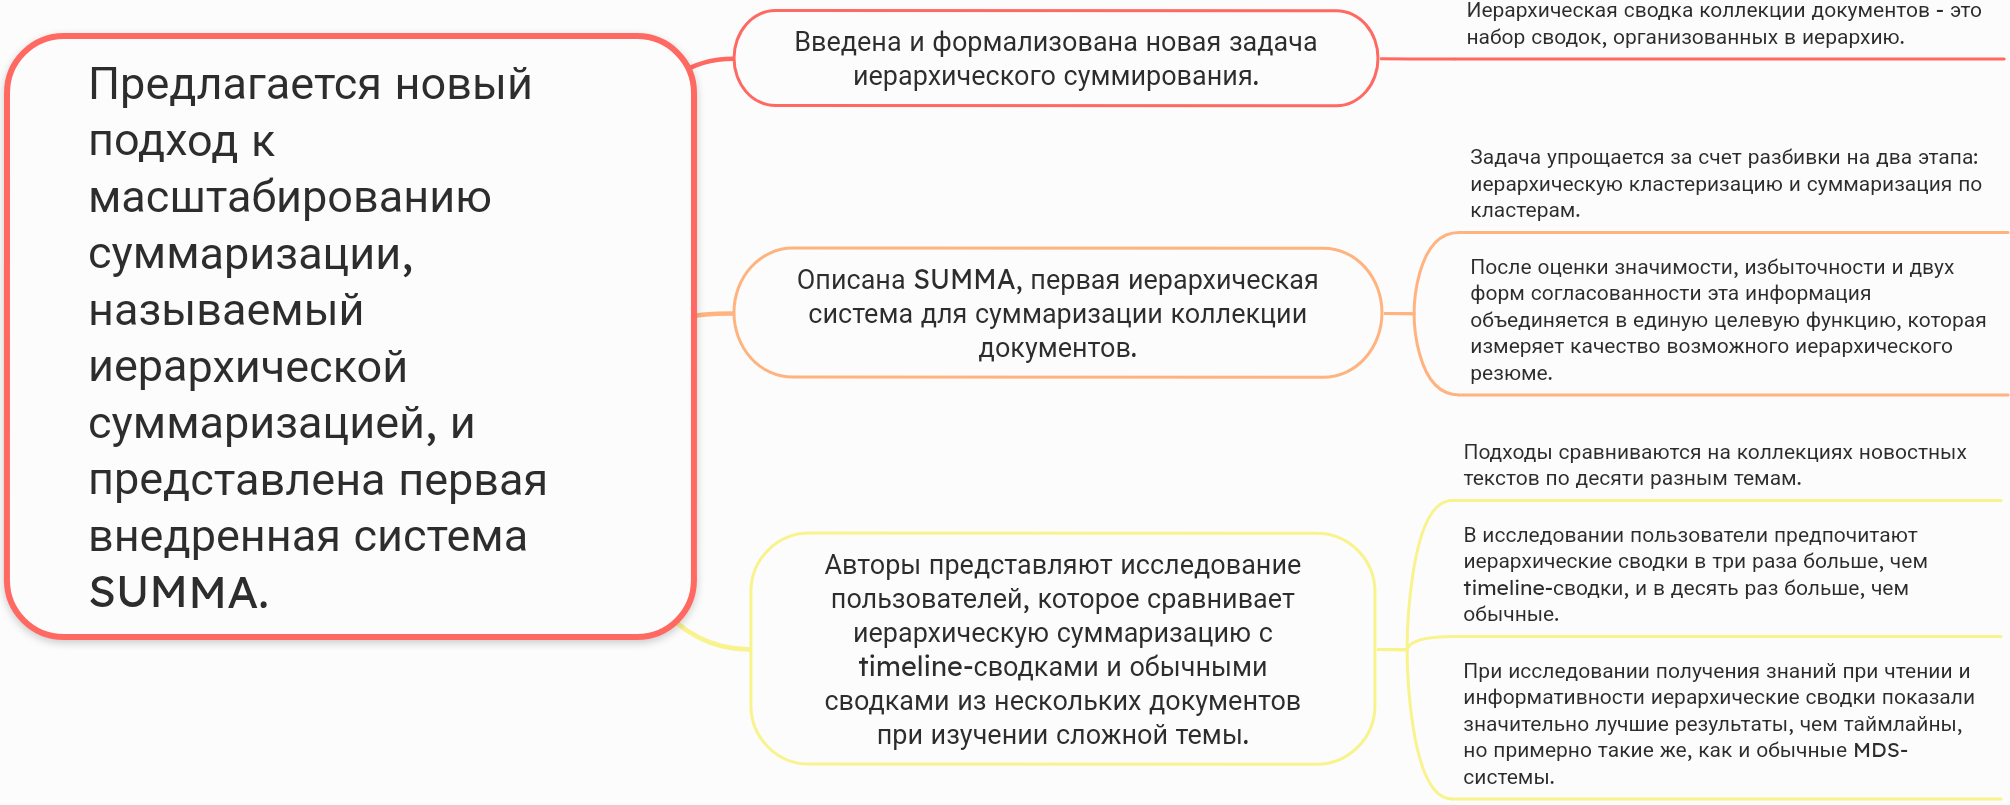
\includegraphics[width=0.8\linewidth]{img/example_map.png}
    \caption{Пример карты по статье об иерархической суммаризации}
    \label{fig:example_map}
\end{figure}

\footnotetext{
        \emph{Christensen J., Soderland S., Bansal G., et al.} Hierarchical summarization: Scaling up multi-document summarization, 2014
    }

\end{frame}

%%%%%%%%%%%%%%%%%%%%%%%%%%%%%%%%%%%%%%%%%%%%%%%%%%%%%%%%%%%%%%%%%%%%%%%%%%%

\begin{frame}{Литература}

\begin{itemize}
    \item \emph{Christensen J., Soderland S., Bansal G., et al.} Hierarchical summarization: Scaling up multi-document summarization, 2014

    \item \emph{Wei Y., Guo H., Wei J.-M., Su Z.} Revealing semantic structures of texts: multi-grained framework for automatic mind-map generation, 2019

    \item \emph{Hu M., Guo H., Zhao S., Gao H., Su Z.} Efficient mind-Map generation via Sequence-to-Graph and reinforced graph refinement, 2021

    \item \emph{Zhang Z., Hu M., Bai Y., Zhang Z.} Coreference graph guidance for mind-map generation, 2024
    
    \item \emph{Guerrero J., Ramos P.} Mind mapping for reading and understanding scientific literature, 2015
\end{itemize}
    
\end{frame}

%%%%%%%%%%%%%%%%%%%%%%%%%%%%%%%%%%%%%%%%%%%%%%%%%%%%%%%%%%%%%%%%%%%%%%%%%%%%

\begin{frame}{Постановка задачи: обычная суммаризация}

\begin{itemize}
    \item Пусть дан документ (или коллекция документов) $\D$~--- упорядоченный набор предложений, составленных из слов некоторого словаря $V$: 
    $$
    \D = \left(s_i\right)_{i=1}^{|\D|},\quad \text{где } \forall i=1,\dots |\D|\quad s_i = \left(w_{ij}\right)_{j=1}^{l_i}, \quad w_{ij}\in V,
    $$
    а также референсная сводка этого документа $\S^*$ и метрика качества $\I: (\S, \D, \S^*) \rightarrow \R$.
    \item Требуется найти отображение $f^*: \D \rightarrow \S$, максимизирующее данную метрику качества $\I$, где $\S = \left(s'_i\right)_{i=1}^{|\S|}$~--- краткая сводка (summary) документа, состоящая из некоторых новых предложений из слов словаря $V$:
    $$
    f^* = \arg\max\limits_{f} \I(f(\D), \D, \S^*).
    $$
\end{itemize}

\end{frame}

%%%%%%%%%%%%%%%%%%%%%%%%%%%%%%%%%%%%%%%%%%%%%%%%%%%%%%%%%%%%%%%%%%%%%%%%%%

\begin{frame}{Постановка задачи: иерархическая суммаризация}

\begin{itemize}
    \item Пусть даны документ $\D$~--- упорядоченный набор предложений из слова словаря $V$, референсная карта $\M^* = (\S^*, E^*)$ и метрика качества $\I: (\M, \D, \M^*) \rightarrow \R$.
    \item Требуется найти отображение $f^*: \D \rightarrow \M = (\S, E)$, максимизирующее данную метрику качества $\I$, где $\M$~--- древовидная \textbf{иерархическая карта} (\textit{интеллект-карта}, \textit{карта знаний}, salient sentence-based mind map), $\S$~--- набор предложений, являющихся вершинами $\M$ и составленных из слов словаря $V$, $E\in \S^2$~--- направленные иерархические связи между предложениями из $\S$, то есть ребра направленного графа $\M$:
$$
f^* = \arg\max\limits_{f} \I(f(\D), \D, \M^*).
$$
\end{itemize}
\footnotetext{
    \emph{Wei Y., Guo H., Wei J.-M., Su Z.} Revealing semantic structures of texts: multi-grained framework for automatic mind-map generation, 2019
    }

\end{frame}

%%%%%%%%%%%%%%%%%%%%%%%%%%%%%%%%%%%%%%%%%%%%%%%%%%%%%%%%%%%%%%%%%%%%%%%%%%

\begin{frame}{Постановка задачи оптимизации промптинга}

\begin{itemize}
    \item Пусть дана выборка документов $\X$, языковая модель $f$, карта-стандарт $\M^*$ для заданной цели создания карты и некоторая метрика качества $\I$. Пусть также задано множество возможных запросов $\Q$, таких что вывод модели для каждого $(\D, Q)\in\X\times\Q$ соответствует требуемому формату, и содержащих формулировку цели, \textit{общую для модели и экспертов} - создателей $\M^*$.
    \item Требуется найти оптимальный запрос $Q^*\in\Q$, такой что вывод модели при входе $(\D, Q^*)$ максимизирует метрику $\I$ по выборке $\X$:
    $$
    Q^* = \arg\max\limits_{Q\in\Q} \frac{1}{|\X|}\sum\limits_{\D\in\X} \I(f(\D, Q), \D, ).
    $$
    \item Для эффективного поиска оптимального запроса (\textit{промптинга}) требуется также задать полное и неизбыточное множество запросов $\Q$ и эффективную \textit{стратегию поиска оптимального запроса} в $\Q$.
\end{itemize}

\end{frame}

%%%%%%%%%%%%%%%%%%%%%%%%%%%%%%%%%%%%%%%%%%%%%%%%%%%%%%%%%%%%%%%%%%%%%%%%%%

\begin{frame}{Многокритериальное оценивание интеллект-карт}

\begin{itemize}
    \item \emph{Этап 1.} Пусть мы имеем сгенерированную моделью по документу $\D$ карту знаний $\M$ и карту-стандарт $\M^*$ по тому же документу, созданную экспертами. 
    \item Требуется определить критерии $\I_k: (\M, \D, \M^*) \rightarrow \R$ для автоматического оценивания интеллект-карт, отражающие интересующие нас аспекты качества генерации иерархического представления $\M$ относительно исходного документа $\D$ и карты-стандарта $\M^*$. 
    \item Мера качества критерия~--- коэффициент корреляции с экспертной метрикой $\I^*_k$ оценки соответствующего аспекта качества по некоторой выборке карт $\X$.
    \item Примеры реальных аспектов качества карты знаний:
    \begin{itemize}
        \item \textit{соответствие цели} генерации карты;
        \item \textit{полнота} карты относительно документа;
        \item \textit{непротиворечивость};
        \item \textit{связность} и \textit{неизбыточность};
        \item \textit{логичность}.
    \end{itemize}
\end{itemize}

\end{frame}

%%%%%%%%%%%%%%%%%%%%%%%%%%%%%%%%%%%%%%%%%%%%%%%%%%%%%%%%%%%%%%%%%%%%%%%%%%

\begin{frame}{Многокритериальное оценивание интеллект-карт}

\begin{itemize}
    \item \emph{Проблема:} количество экспертных карт и скорость их создания сильно ограничены, нужно научиться оценивать карты без стандартов. 
    \item \emph{Этап 2.} Пусть мы имеем только документ $\D$ и сгенерированную по нему моделью карту знаний $\M$.
    \item Требуется определить критерии $\I_k: (\M, \D) \rightarrow \R$, отражающие качество генерации иерархического представления $\M$ исходного документа $\D$ самого по себе, без сравнения с другими картами. 
    \item Мерой качества автоматического критерия, помимо степени скоррелированности с экспертными критериями, является также результат оценивания с помощью него экспертных карт $\M^*$, принимаемых за стандарт.
\end{itemize}

\end{frame}

%%%%%%%%%%%%%%%%%%%%%%%%%%%%%%%%%%%%%%%%%%%%%%%%%%%%%%%%%%%%%%%%%%%%%%%%%%

\begin{frame}{Методы исследования}
    
\begin{itemize}
    \item Метод сбора данных~--- собственная работа и работа привлеченных экспертов по построению иерархических сводок научных статей.
    \item Метод агрегации экспертных мнений: проведение научных семинаров в формате обсуждения интеллект-карт по статьям с последующим построением общей карты. Пусть мы собрали $N$ экспертов, тогда на выходе мы имеем по каждой обработанной статье $N+1$ карт, одна из которых является золотым стандартом для данной статьи.
    \item Метод отбора критериев: сбор на вышеупомянутых семинарах экспертных оценок аспектов качества сгенерированных искусственно интеллект-карт по рассматриваемым статьям, затем анализ корреляций экспертных оценок и значений автоматических критериев.
\end{itemize}

\end{frame}

%%%%%%%%%%%%%%%%%%%%%%%%%%%%%%%%%%%%%%%%%%%%%%%%%%%%%%%%%%%%%%%%%%%%%%%%%%

\begin{frame}{Этапы эксперимента}

\begin{itemize}
    \item \textit{Текущий этап:} отработка методологии построения интеллект-карт по научным статьям с привлечением экспертов для сбора тестовых данных и валидации метрик качества;
    \item Разработка и тестирование стратегий промптинга БЯМ для задачи иерархической суммаризации, максимизирующих выбранные метрики качества по полученным данным;
    \item Полномасштабное тестирование современных БЯМ на полученных данных при помощи выработанных стратегий промптинга и анализ результатов генерации.
\end{itemize}

\end{frame}

%%%%%%%%%%%%%%%%%%%%%%%%%%%%%%%%%%%%%%%%%%%%%%%%%%%%%%%%%%%%%%%%%%%%%%%%%%

\end{document} 